\documentclass[12pt]{article}
\usepackage{latexsym}
\usepackage{setspace}
\usepackage{graphicx}
\graphicspath{ {/} }

\doublespacing

\parskip=3pt

\setlength{\textheight}{8.5in}
\setlength{\textwidth}{6in}
\setlength{\topmargin}{0in}
\setlength{\oddsidemargin}{0in}
\setlength{\evensidemargin}{0in}

\def\inst#1{$^{#1}$}

\title{Digital Privacy and Cryptography}

\author{
	Dallas J. Fraser\inst{1}
}

\begin{document}
\maketitle

\begin{center}
{\footnotesize

\inst{1}, Department of Physics and Computer Science, Wilfrid Laurier 
University, November 22, 2014}

\end{center}

\begin{abstract}
Do people care about digital privacy and how can cryptography keep digital information private
\end{abstract}

\noindent{\em Keywords}: Digital Privacy, Cryptography, Privacy enhancing technologies (PET),

\clearpage

\section{History of Growth and Loss of Privacy}\label{sec:history}

Digital privacy refers to the collection and security of digital information that is quite personal in nature. A brief history of digital information helps show how digitial privacy has been changing recently. The growth of the Internet in the 1990's raised communication to a global level. It has changed society in many different aspects such as culture, communication, games, and even business. New industries were created by the internet, lead by new companies such as Google, Apple, and eventualy Facebook.

The development of databases, the growth of mobile industry  and the increase usage of the Internet have resulted in a huge collection of personal data. More companies are moving their Information Techonology to the cloud and are creating Data Centers which store an inconceivable amounts of data. Facebook has claimed that they have over a 100 petabytes of photos and video \cite{Wallbank}. This along with a strong developer community has lead to anyone being able to create a web application. There are tons of web based hosting companies such as Heroku which allows any to publish their web application easily. New technologies are created yearly for all kinds of web development. There are over 250,000 web related repositories on Github alone. There are numerous plugins to enabling your web application to be integrated with numerous social media websites such as Twitter and Facebook. The Internet has provided connections across the world but these connections have some issues.

\section{Do People Care?}\label{sec:demand}

People are constantly giving out personal information such as email, address, and credit card daily through various websites. All kinds of information is being tracked when browsing through Google analytics. With all this information being shared and stored everyday, are people concerned with its security and their privacy?

A recent study performed by Pew Research Center had a study on ``Public Perceptions of Privacy and Security in the Post-Snowden Era''. The two most intersting results were ``80 percent of those who use social networking sites say they are concerned about third parties like advertisers or businesses accessing the data they share on these sites'' and ``70 percent of social networking site users say that they are at least somewhat concerned about the government accessing some of the information they share on social networking sites without their knowledge.'' \cite{Madden}. This shows that the majority of people are concerned about privacy. These concern is most likely founded upon the recent news reports such as Snowden reports and the large collection of celebrity hacks. A lack of understanding of how these techonogies work and the security behind lends a hand as well.

The Pew study was based in America but Canadians have similar feelings. Taking a look at Canadian politics where the privacy laws are being challenged. ``As organizations find new ways to profit from personal information, the risks to privacy are growing exponentially,'' says Commissioner Stoddart \cite{PrivacyCommissioner}. Europe is more concerned thatn North America and recently challenged search companies especially search giant Google. ``The European Parliament has passed a historic vote to break up US tech giant Google.''\cite{Cook}. This is on top of the fact that Google and EU are in the middle of a four year long dispute about anti-trust laws.

It is evident that people are concerned about digital privacy. However, this seems to contradict the behaviour of people, where countless of private photos are uploaded and personal messages sent everyday. ``Most say they want to do more to protect their privacy, but many believe it is not possible to be anonymous online''\cite{Madden}. Most consumers feel that protecting their information is too difficult and their rights as a consumer are non-existence. 

\section{Digital Privacy Supply}\label{sec:supply}

The developer community and business are one creating the applications which collect the data. Increases in techonologies allows for developers to create and publish webites in a short time. This is evident in hackathons where website are created in a weekend. Engineering processes are evolving to help encourage rapid change and this is seen through Agile development. Is security is a major concern for businesses in this process and do they meet consumer demands?

Business are driven by profit and will lok to way to maximize profit in any manner if there is not government intervention. Sadly there is a lack of legislation dealing with the Internet. This is largely due to the how fast these techonologies have grown and how slow the political systems moves. Most of contract law is obsolete when it comes to the Internet and Internet transactions. Canada's Anti-Spam Legislation (CASL) which was passed in Decemeber 2010 but not enforced until July 1, 2014 \cite{FastFacts}. It took about a decade and a half to create a spam law and another four years to implement it. The lack of legislation allows for companies to freely deal with their data, and user' agreements with little government interference. The goverment is doing little to ensure digital privacy and in certain cases in exploiting personal information in the name of security. A recent example is the N.S.A complaint about Apple's Iphone encryption of data where the user's password was used to encrypt the data \cite{Schneier}. Encryption is more of a hassle and back doors make their job much easier.

All business have the incentive to improve profit and without external incentives will strictly focus on profits. The two greatest external forces on corporations are the government and public opinion. The government's pressure on companies is non-existence and what force that is present is outdated. The public is less concerned about with drawbacks of the data privacy and more concerned with the benefits of the application. Most people ask what can it do for me instead of how does it work and what security measures are in place? The lack of incentives have lead to business tending to focus more what profit can be produced from personal data and not the long term impact it could have. There is a lack of research done by the companies producing these techonologies on the users. The negative side effects are not taken into consideration during the design process. Security is usually an after thought and privacy is never considered. This is evident in a recent study done by Cisco Canada in which they found ``40 per cent of about 500 firms surveyed had security strategies'' \cite{Blackwell}. Just last week, Sony was hacked where a significant amount of employee information was leaked. Their are estimates of ``100 terabytes of data'' leaked containing information such as ``list of employee salaries and bonuses; Social Security numbers and birth dates; HR employee performance reviews, criminal background checks and termination records'' \cite{Zetter}.

The demand of digital privacy is greater than the current supply of security. The lack of legislative and consumer pressures have prevented companies from increasing their level of security. This has resulted in insecure websites and vulnerable private information. 

\section{Need for Change}\label{sec:change}
The lack of security is a concern for most people. A lot of the personal information is freely shared by the consumers of social media. Examining some the issues related to digital privacy will provide incentive to change.

The culture change started by the Internet has brought new social issues. Now a citizen is evaluated by their on-line social interaction. Companies will use Facebook, LinkedIn and Google to screen out potential candidates. Employers need to monitor the social lives closely because of this. One cyber attack can greatly damage one reputation and may threaten their employment or even their employability. The other thing is the Internet does not forget about one's past. A good example of this is the recent firing of a Quebec teacher. ``he availability on the Internet of erotic films in which she acted created an entirely new context that was not ideal for our students'' \cite{Peritz} was the reason for her dismissal. This problem will only get larger as more information is stored and moved into an age where all data becomes digitalized.

The new buzz in the business world is big data and processing big data for applications. The applications are used by business to make decision and to help better market their product. There is a big push for all companies to collect data and analyzing this data to get ahead. Their are large claims by people of all the potential including big data making people happy \cite{Banayan}. The collection of this data has little regulations and with an increasing financial incentive it can or may cause some business to collect this information in unethical ways. The other problem is the over confidence in this new field. Micheal Jordan a Professor at the University of California stated that ``When you have large amounts of data, your appetite for hypotheses tends to get even larger. And if it’s growing faster than the statistical strength of the data, then many of your inferences are likely to be false. They are likely to be white noise.'' \cite{Gomes}. Google Flu Trends is a system Google has developed for tracking the flu. ``Google Flu Trends is often held 
up as an exemplary use of big data''. \cite{Lazer}. It was reported that ``GFT was predicting more than double the proportion of doctor visits for influenza- like illness (ILI) than the Centers for Disease Control and Prevention (CDC),'' \cite{Lazer}. This is a good case example of how big data does not have all the answers and is a field that needs improvement and reasearch. Over confidence in it could lead to costly mislead decisions based on ``big data hubris'' \cite{Lazer}.

The rise of social reputation and impact on lives raised the need for security. The lure of big data entices companies to quickly implement big data storage and collection. The lure of big data possibilites sometimes overshadows security and digital privacy. Security and digital privacy should be more important that big data and its applications. ``If I have no principles, and I build thousands of bridges without any actual science, lots of them will fall down, and great disasters will occur''.(Micheal Jordan)\cite{Gomes}

\section{Ways to  Change}\label{sec:developers}
It is clear that security and digital privacy need to be focused and strengthened. A developer needs to recognize this during the design of their system. They need to build into their system ways users can stay annonymous or delete private information when requested. Digital privacy should be the standard when creating web applications and not a feature.

There a wide range of Private Enhancing techniques using Crypotgraphy. This paper will focus on Private Digital Credentials, Type X remailers, Onion Routing, and Transport Layer Security while highlighting on how these can allow for digital privacy. A few defintions to establish are anonymity and pseudonymity. Anonymity systems are built to make one-way communication while getting information private while pseudonymity are built to allow for two-way communcation by using a pseudonym to help keep information private. \cite{GoldbergTwo}

\section{Private Digital Credentials - Blind Signatures}\label{sec:PDC}
Digital Credentials are just information that can be used to qualify a certain property. One Example would be a Laurier Digital Diploma whichs qualifies that a person graduated from Laurier University.  Private Digital Credentials are used as a way to qualify but keep anonymity for the presenter. The idea was first proposed by Daivd Chaum in 1985 \cite{Chaum}. He introduces the idea of unconditional untraceabile payments which used signatures called ``blind signatures''\cite{Chaum}. 

David Chaum uses the analogy of Private Digital Credentials to the use of a carbon-paper-lined envelope. Once the letter is inserted into the envelope any mark on the exterior of the envelope will be applied to the letter. A person could sign the letter without ever seeing the letter. The proposed system is one in which a person uses blind signatures to receive the banks authentication of a dollar and subtracts the amount from the account. The banks uses the same signatures for all transactions. The bank can verify any letter has the bank's signature but cannot identify which envelope the letter came from.

The steps of the system start by the user creating a note number called $n$ which is a random number. The users then creates a second random number  $r$. The note number $n$ is then blinded by combing $n$ with $r$. This is done mathematically by $n * r^b$ where $b$ is the bank's public power which equates to one dollar. The blinded note is then transferred to the bank. The banks signs the blinded note by using its private power $\overline{b}$. The result is return and the signed note number is obtained by dividing out the $r$ to obtain $n^{\overline{b}}$. The note can be verified that is a signed special number.

The banks needs to keep track of transactions to ensure that no note has been used twice. This is done by having a list of all accepted transactions. A transaction is only allowed if not part of the list and has the appropriate signature. The underlying digital signature techniques make it difficult for anyone to forge the bank's signature $\overline{b}$ \cite{Chaum}. If $r$ is not disclosed then the transcation deposit cannont be linked to the withdrawel.

The most common uses of blind signatures are digital cash and voting protocols. Digital cash is related to private digital credentials. David Chaum's analogy makes this quite clear. Any system which implements private digitial credentials could also be used for a digital cash system. Digital cash would be a great way to keep personal financial information private. Credit card companies track most on-line transcations and with digital cash it could help users retain anonymity. One real life example is Credentica, who have a technology called U-Prove which can be used to provide digital privacy.

\section{Type X Remailers}\label{sec:type-x}
What is it?
The initial focus on prviacy dealt with email. One initial approach was have a third party remove all identifying information and then forward the message to the intended recipent. The other approach was to create a fake email with false information sometimes refer to as pseudonym. Hence people starting creating systems to reduce the work of the user trying to protect their information.

These anonymous remailer which aim to allow users to allow for e-mail communcations without losing privacy. There are four differ Versions of Type X Remailers, Type O, Type I, Type II and Type III with Type III providing the most functionality. All the different versions work differently where some are anonymity systems and others are pseudonym systems.

Type 0 remailer was also called anon.penet.fi \cite{GoldbertTwo}. It allowed for pseudonym commuication by having a table the matched the email addresses to the pseudonym. The recipent could respond and the Type 0 remailer would use the table to send the email back to real mail address. The service was shut down and only offers minimal security \cite{GoldbertTwo}.

Type I was also known as Cypherpunk was designed to address the security issues of Type 0. The major changes included no pseudonyms, encrypt/decrypt messages, and uses chaining. Chaining is the idea of sending the message through various remailers to make it more difficult to trace through. Type I was also combined with encryption to make it more difficult to intercept and read the intended message. Type II which was also known  Mixmaster added in more security to deal with certain types of eavesdroppings attacks such as correlation. 

Type III is also known as Mixminion and had its first release in 2002. Mixminion aimed to support pseodonymity in which Type II had poor support\cite{GoldbertTwo}. The project had its own git on Github which has not been updated since 2011. According to their design document which can be found on their website, the designers had the following goals simplicity for clients, simple to deploy, and drop packets-level compatibility with Mixmaster (Type II).  Mixminon uses a free-route mix but does not implement reusable reply blocks.

Anonymous Remailers can be used to send communications anonymously. However Type III  has been said to not be trusted for anonymity \cite{GoldbertTwo}. The previous version have their technical issues. This details would need to be sorted out before this techonlogy can be confidently replied upon.

\section{Onion Routing}\label{}
Onion Routing is a system that allows a user to commuicate with servers while maintaining anonymity. The name is derived from how the system peels away encryption similar to the peeling of an onion. The system to use this idea was the Onion Router and the idea was published in 1998 \cite{Reed}. 

The simple idea of Onion Routing is creating an indirect path between nodes starting at the user's node and ending at the recipents. Each node in the path does not the recipents but rather just the next node in the path. Each node does not know the path due to the way the packet is encrypted. Each node removes a level of encryption and to determine which node to pass to. This path may be used so the recipent can respond which allows of pseudonymous communications.

The anonymous connection is established by the onion which is described as multi-layered data structure. It layer of the onion has a version, back part, forward part, destination port, desistnation address, expiration time, and key seed material. The back part determines what type of encryption should be applied to data moving backwards and forward part is the type of encryption that should be applied to data moving forwards.  Onion Router uses various forms of encryption such as $DES$ $OFB$ and $RC4$\cite{Reed}. The desitnation port and address is the information about the next address with 0 being used to signal the exit node. Key seed material stores three keys $k_1, k_2, k_3$ which are produced using $SHA$. The keys are used when encrypting with $DES$ and $RC4$. Each data node is of size 1024-bits mainly due to Onion Routing uses $RSA$ public key cryptography.

The creators of Onion Routing designed it to prevent traffic analysis. This helps users be able to prevent someone from determining the private information. The creators even discussed applications of Onion Routing such as email, web browsing, digital cash, and a few others\cite{Reed}. Tor is the successor to the Onion Router and can be used for browsing along with other things. There are wide range of software and services that can be found on Tor Project webpage including Tor browser and even Orbot which is Tor for Android device. There are a few criticisms of Tor such as slow web browsing speed \cite{GoldbertTwo}.

\section{Transport Layer Security}\label{sec:tls}

Transport Layer Security (TSL) protocol is the successor of Secure Socket Layer protocol. It is supported in all modern browswers such as Chrome, Firefox, and Internet Explorer. TLS is a protocol which ensures information is transmitted securly. Transport Layer Security was designed to prevent eavesdropping and ensures information is not intercepted and changed during transmission \cite{Sidhpurwala}.

The protocol first exchanges keys using a key exchange. The data is then encrypted using a specified encyrption function such as AES. A message authencating code (MAC) is also created. The encyrpted text and th MAC is sent. The encyrption does not allow for eavesdropper to read the intended message. The MAC does not allow the user to intercept the message and change it.

The client will request to use Transport Layer Security and which initiates the Transport Layer Security handshake \cite{Sidhpurwala}.  The Transport Layer Security handshake has the six following steps:
\begin{enumerate}
	\item ClientHello: The client initial message that specifies supported Transport Layer Security versions, cipher suits, and compression methods. 
	\item ServerHello: The server responsed with a message that specifies with version of Transport Layer Security, cipher suit, and compression method to use. The message also contains an a random generated string $r$.
	\item ClientKeyExchange: The client generates a secret $s$ using the server public key. The client than transmits a record called ClientKeyExchange along with the secret $s$. Client and server use $r$ and $s$ to create a Master Secret. 
	\item ChangeCipherSpec: The client then sends a message which signals all information will be encrypted. The client then proceeds to send the encrypted message and authentication. 
	\item ChangeCipherSpec(response): The server response to the clients message.
\end{enumerate}

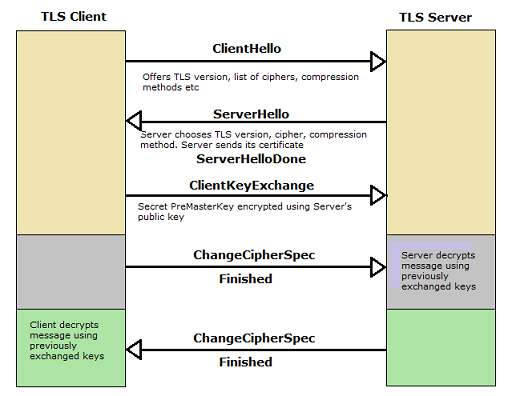
\includegraphics{tls-handshake}
 
 Transport Layer Security is a widely used. Transport Layer Security is a good example of when standards are created then people will follow them. It is not difficult to enable a web application to support Transport Layer Security through various libraries such as OpenSSL. There are still problems with TSL/SSL and this was shown recently through the HeartBleed Bug. HeartBleed was a good example of the lack of funding applied to security budgets.

\section{Companies doing Security Right}\label{sec:real-life}
Wickr is a new messenger which is available on Google Play store, Apple App Store, and even for desktop. It is uses peer-to-peer encryption and enables users to send encrypted messages.  According to its website it uses hashed all device information with SHA256 and encrypts all data with AES256. The Wickr server only handles encrypted messages and delete the message upon delivery. The server also never directly interacts with devices identifiers but onlt the hashes of them. Wickr has received four and a half stars on the Apple store from 80 different ratings and has a similar rating on the Google Play store. 

Blackberry
A Canadian based company focusing on mobile communications. It once had was the standard smart phone in Canada but quickly consumers switch to over to Apple and Android. Their were rumours about Blackberry being possible bought by various companies. The company hired a new C.E.O. who change the focus away from the consumer market. Blackberry now focuses on one of its strengths security and even Preseident Obama uses one.\cite{Marks} Blackberry is a good example of a company focusing on the under suplied market of security. The stock price seems to be trending upwards.


\section{Conclusion}\label{sec:conclusion}
There are rising concerns of consumers about privacy issues. Security is often over-shadowed by usability and convenient apps. Legislation is starting to approached these issues related to digital privacy and setting expectations on business. The business world is focused too much on big data and profitting from it however there are some who are focusing on security. The market for secure applications will grow and cryptography will allow for a consumer to keep digital privacy. Hopefully the supply of digital privacy will meet the demand of it.

\begin{center}
{\bf Acknowledgement}
\end{center}
This work was done by author D.J.F. in partial fulfillment of the course requirements for CP460: Applied Cryptography in the Department of Physics and Computer Science at Wilfrid Laurier University.

\clearpage
\singlespace
\begin{thebibliography}{99}
\bibitem{Albergotti}
	Albergotti, R. (2014, November 13). Facebook Gives Its Privacy Policy a Makeover. Retrieved November 16, 2014, {\sl http://blogs.wsj.com/digits/2014/11/13/facebook-gives-its-privacy-policy-a-makeover/}
\bibitem{Doctorow}
	Doctorow, C. (2014, November 12). Peak indifference-to-surveillance. Retrieved November 14, 2014, {\sl http://boingboing.net/2014/11/12/peak-indifference-to-surveilla-2.html}
\bibitem{Gomes}
	Gomes, L. (2014, October 20). Machine-Learning Maestro Michael Jordan on the Delusions of Big Data and Other Huge Engineering Efforts. Retrieved October 26, 2014, {\sl http://spectrum.ieee.org/robotics/artificial-intelligence/machinelearning-maestro-michael-jordan-on-the-delusions-of-big-data-and-other-huge-engineering-efforts}
\bibitem{Lawton}
	Lawton, V. (2013, May 23). New privacy challenges demand stronger protections for Canadians. Retrieved October 14, 2014
\bibitem{Lazer}
	Lazer, D., Kennedy, R., King, G., and Vespignan, A. (2014, March 14). The Parable of Google Flu: Traps in Big Data Analysis. Retrieved November 17, 2014.
\bibitem{Madden}
	Madden, M. (2014, November 12). Public Perceptions of Privacy and Security in the Post-Snowden Era. Retrieved November 15, 2014, {\sl http://www.pewinternet.org/2014/11/12/public-privacy-perceptions/}
\bibitem{Notley}
	Notley, T. (2014, August 4). Why digital privacy and security are important for development. Retrieved October 14, 2014, {\sl http://www.theguardian.com/global-development/poverty-matters/2011/aug/04/digital-technology-development-tool}
\bibitem{Nowak}
	Nowak, P. (2014, June 21). In era of revelation, privacy more important than ever. Retrieved October 14, 2014, {\sl http://business.financialpost.com/2012/06/21/in-era-of-revelation-privacy-more-important-than-ever}
\bibitem{Roughhol}
	Roughol, I. (2014, November 19). Uber's Privacy Scandal Is a Failure of Culture. Retrieved November 19, 2014, {\sl
	https://www.linkedin.com/today/post/article/ubers-privacy-scandal-failure-isabelle}
\bibitem{Schneier}
	Schneier, B. (2014, October 6). IPhone Encryption and the Return of the Crypto Wars. Retrieved November 23, 2014, {\sl https://www.schneier.com/blog/archives/2014/10/iphone \textunderscore encrypti \textunderscore 1.html}
\bibitem{Solove}
	Solove, D. (2014, November 12). People Care About Privacy Despite Their Behavior. Retrieved November 13, 2014, {\sl https://www.linkedin.com/today/post/article/20141112171953-2259773-people-care-about-privacy-despite-their-behavior}
\bibitem{WallBank}
	Wallbank,P. How much server space do Internet companies need to run their sites? {\sl http://paulwallbank.com/2012/08/23/how-much-server-space-do-internet-companies-need-to-run-their-sites/} (2012)

\bibitem{FastFacts}
	Fast Facts. (2013, December 4). Retrieved November 23, 2014, {\sl from http://fightspam.gc.ca/eic/site/030.nsf/eng/h\textunderscore00039.html}

\bibitem{PrivacyCommissioner}
	Lawton, V. (2013, May 23). New privacy challenges demand stronger protections for Canadians. Retrieved October 14, 2014, from https://www.priv.gc.ca/media/nr-c/2013/nr-c \textunderscore 130523\textunderscore e.asp

\bibitem{Cook}
	Cook, J. (2014, November 27). The European Parliament Just Voted To Break Up Google Read more: Http://www.businessinsider.com/european-parliament-voted-to-break-up-google-2014-11ixzz3KhLx0CEU. Retrieved November 28, 2014, from http://www.businessinsider.com/european-parliament-voted-to-break-up-google-2014-11

\bibitem{Blackwell}
	Blackwell, R. (2014, December 2). Many Canadian firms are unprepared to face cybersecurity attacks: Study. Retrieved December 2, 2014, from http://www.theglobeandmail.com/report-on-business/smaller-canadian-firms-less-prepared-for-threat-of-cyberattack/article21857498/

\bibitem{Peritz}
	Peritz, I. (2014, October 20). Montreal teacher, 73, loses job over film nudity more than 40 years ago. Retrieved December 2, 2014, from http://www.theglobeandmail.com/news/national/montreal-teacher-73-loses-job-over-film-nudity-more-than-40-years-ago/article21183669/

\bibitem{Banayan}
	Banayan, A. (2014, November 4). 2 Ways Big Data Can Make You Happier. Retrieved November 5, 2014, from https://www.linkedin.com/pulse/article/20141104090919-80844253-2-ways-big-data-can-make-you-happier?trk=tod-home-art-list-large\textunderscore0

\bibitem{Zetter}
	Zetter, K. (2014, December 3). Sony Got Hacked Hard: What We Know and Don’t Know So Far. Retrieved December 3, 2014, from http://www.wired.com/2014/12/sony-hack-what-we-know/

\bibitem{Goldberg}
	Goldberg, I., Wagner, D., and Brewer, E. (1997, January 21). Privacy-enhancing technologies for the Internet. Retrieved December 3, 2014, from http://www.cypherpunks.ca/~iang/pubs/privacy-compcon97.pdf

\bibitem{GoldbergTwo}
	Goldberg, I. (2007, December 1). Privacy Enhancing Technologies for the Internet III: Ten Years Later. Retrieved December 3, 2014, from http://www.cypherpunks.ca/~iang/pubs/pet3.pdf

\bibitem{Chaum}
	Chaum, D. (1985, October 10). Security without identification: Transaction systems to make big brother obsolete. Communications of the ACM, 1030-1044.

\bibitem{Reed}
	Reed, M., Syverson, P., and Goldschlag, D. (1998, January 1). Anonymous Connections and Onion Routing. Retrieved December 5, 2014, from http://www.onion-router.net/Publications/JSAC-1998.pdf

\bibitem{Marks}
	Marks, G. (2014, March 4). Here's Why You May Be Buying BlackBerry Again. Retrieved December 5, 2014, from http://www.forbes.com/sites/quickerbettertech/2014/03/04/heres-why-you-may-be-buying-blackberry-again/

\bibitem{Sidhpurwala}
	Sidhpurwala, H. (2013, July 24). Transport Layer Security. Retrieved December 6, 2014, from https://securityblog.redhat.com/2013/07/24/transport-layer-security/
\end{thebibliography}

\end{document}

